% This must be in the first 5 lines to tell arXiv to use pdfLaTeX, which is strongly recommended.
% \pdfoutput=1

\tracinggroups=1
\tracingnesting=2

\documentclass[10pt]{article}

\usepackage{latexsym}
\usepackage{hyperref}
\usepackage{enumitem}
\usepackage{setspace}
\usepackage{wrapfig}
\usepackage[center,format=plain,
            labelfont={bf,it},
            textfont=it]{caption}
\usepackage{graphicx}
\graphicspath{ {./figures/} }

% Syntax highlighting
\usepackage{minted}
\usepackage{tcolorbox}
\usepackage{etoolbox}
% \setminted{frame=single}
\BeforeBeginEnvironment{minted}{\bigskip\begin{tcolorbox}}
\AfterEndEnvironment{minted}{\end{tcolorbox}\bigskip}

\setstretch{1.2}

% For proper rendering and hyphenation of words containing Latin characters (including in bib files)
\usepackage[T1]{fontenc}
% For Vietnamese characters
% \usepackage[T5]{fontenc}
% See https://www.latex-project.org/help/documentation/encguide.pdf for other character sets

% This assumes your files are encoded as UTF8
\usepackage[utf8]{inputenc}

% This is not strictly necessary, and may be commented out.
% However, it will improve the layout of the manuscript,
% and will typically save some space.
\usepackage{microtype}

% This is also not strictly necessary, and may be commented out.
% However, it will improve the aesthetics of text in
% the typewriter font.
\usepackage{inconsolata}


% Margins: see http://practicaltypography.com/page-margins.html and
% http://practicaltypography.com/line-length.html
% We're aiming for 80-ish characters per line.
\usepackage[inner=1.4in,outer=1.4in,top=0.75in,bottom=1in,
            footnotesep=11bp,
           ]{geometry}

\usepackage[
    hyperref=true,
    natbib=true,
    style=alphabetic,
    backend=biber]{biblatex}

\NewBibliographyString{urlrestricted}
\DefineBibliographyStrings{english}{
  urlrestricted = {restricted access},
  }

\DeclareFieldFormat{url}{%
  \mkbibacro{URL}\addcolon\space
  \url{#1}%
  \iffieldannotation{restricted}
    {\space
     \mkbibbrackets{\bibstring{urlrestricted}}}
    {}}

\usepackage{filecontents}
\begin{filecontents}{\jobname.bib}

@misc{Anchors,
    author = {Gregory Sanders},
    title = {Ephemeral Anchors: Fixing V3 Package RBF against package limit pinning},
    url = {https://lists.linuxfoundation.org/pipermail/bitcoin-dev/2022-October/021036.html},
    year = {2022},
}

@misc{OptechPkgRelay,
  author = {Various},
  title = {Bitcoin Optech: Package Relay},
  url = {https://bitcoinops.org/en/topics/package-relay/},
}

@misc{OptechAnchors,
  author = {Various},
  title = {Bitcoin Optech: Anchor Outputs},
  url = {https://bitcoinops.org/en/topics/anchor-outputs/},
}

@misc{Revault,
  author = {Revault},
  title = {Revault},
  url = {https://revault.dev},
}

@misc{CTV,
  author = {Jeremy Rubin},
  title = {BIP 119: CHECKTEMPLATEVERIFY},
  url = {https://github.com/bitcoin/bips/blob/master/bip-0119.mediawiki},
  year = {2020},
}

@misc{ElementsScript,
  author = {Sanket Kanjalkar},
  title = {Elements Taproot Introspection Opcodes},
  url = {https://github.com/ElementsProject/elements/blob/master/doc/tapscript_opcodes.md},
  year = {2021},
}

@misc{Sponsors,
  author = {Jeremy Rubin},
  title = {A Replacement for RBF and CPFP: Non-Destructive TXID Dependencies for Fee Sponsoring},
  url = {https://lists.linuxfoundation.org/pipermail/bitcoin-dev/2020-September/018168.html},
  year = {2020},
}

@misc{Cov,
  author = {Malte Möser, Ittay Eyal, and Emin Gün Sirer},
  year = {2016},
  title = {Bitcoin Covenants},
}

@misc{APO,
  author = {Christian Decker, Anthony Towns},
  title = {BIP-118: SIGHASHANYPREVOUT for Taproot Scripts},
  year = {2018},
  url = {https://github.com/bitcoin/bips/blob/master/bip-0118.mediawiki},
}

@misc{OPTX,
  author = {Rusty Russell},
  title = {OPTX: generalized covenants reduced to OPCHECKTEMPLATEVERIFY},
  year = {2022},
  url = {https://lists.linuxfoundation.org/pipermail/bitcoin-dev/2022-May/020450.html},
}

@misc{Bishop,
  author = {Bryan Bishop},
  title = {Bitcoin vaults with anti-theft recovery/clawback mechanisms},
  year = {2019},
  url = {https://lists.linuxfoundation.org/pipermail/bitcoin-dev/2019-August/017229.html},
}

@misc{BishopCode,
  author = {Bryan Bishop},
  title = {python-vaults},
  year = {2020},
  url = {https://github.com/kanzure/python-vaults},
}

@misc{OBeirne,
  author = {James O'Beirne},
  title = {simple-ctv-vault},
  year = {2022},
  url = {https://github.com/jamesob/simple-ctv-vault},
}

@misc{APOVaults,
  author = {Antoine Poinsot},
  title = {simple-anyprevout-vault},
  year = {2022},
  url = {https://github.com/darosior/simple-anyprevout-vault},
}
\end{filecontents}
\addbibresource{\jobname.bib}

% \begin{document}
%     Hallo world \\
%     \cite{einstein}
%     \printbibliography
% \end{document}


% If the title and author information does not fit in the area allocated, uncomment the following
%
%\setlength\titlebox{<dim>}
%
% and set <dim> to something 5cm or larger.

\author{James O'Beirne \\
  \texttt{james.obeirne@gmail.com}
\and
  Brian Langel \\
  \texttt{brian.langel@nydig.com} \\}

\date{\today}
\title{Vaults and Covenants}

\begin{document}

\newcommand{\ctv}{\texttt{OP\textunderscore{}CHECKTEMPLATEVERIFY}}
\newcommand{\opv}{\texttt{OP\textunderscore{}VAULT}}
\newcommand{\opuv}{\texttt{OP\textunderscore{}UNVAULT}}
\newcommand{\spk}{\code{scriptPubKey}}
\newcommand{\code}[1]{\texttt{#1}}


\maketitle
\begin{abstract}

  Vaults are a technique for substantially reducing the risk of Bitcoin management. In
  this paper, we examine their relationship to different covenant implementations. We
  survey the vault implementations that are currently usable, as well as those that
  would be possible only with proposed consensus updates (e.g. \ctv{}). 

  A new approach, \opv{}, is presented which avoids the pitfalls of a general
  covenant proposal while still allowing the covenant-like behavior necessary for a
  featureful vault implementation. The design assumes the deployment of package relay
  and ephemeral anchors for dynamic fee management, but allows for different fee
  management approaches should they come. It allows batching vault operations, partial
  unvaultings, dynamic withdrawal targets, and recursive deposits.

\end{abstract}

\section*{Introduction}

Custodying bitcoin is notoriously difficult. It is roughly equivalent to
another task famous for its trail of bodies: keeping sensitive data accessible but out
of unauthorized reach. Luckily, due to the unique programmability of Bitcoin script,
custodians do not necessarily have to rely solely on the Sisyphean task of key
management.

In Bitcoin, a \emph{covenant} is a constraint put on how a coin can be spent on the
basis of its spending transaction, above and beyond the traditional
requirements of satisfying a one-time unlocking script. Covenants can be written in
such a way that they express recursive constraints on outputs, so that the effective
period of covenant enforcement can span an arbitrary number of transactions. 

Currently there is no way to enforce a covenant ``on chain,'' but there are many
pending proposals for how to modify Bitcoin's validation rules to allow for this
functionality. Proposals can be divided into two kinds:

\begin{itemize}
  \item \textbf{limited}: where the state machine of possible transactions within the lifecycle
    of a covenant is predetermined and therefore bound (e.g. \cite{CTV}, \cite{APO},
    \cite{OPTX}), and

  \item \textbf{general}: where the state machine is expressed within Bitcoin script,
    and can reapply itself indefinitely, making it potentially unbounded (e.g. \cite{ElementsScript}).

\end{itemize}

Vaults are an especially useful kind of covenant that give Bitcoin users
operational simplicity during expected use, but heightened security in light of an
attack. When they were originally presented in \cite{Cov}, a vault was defined as a
simple covenant that ensured that the spend of a coin was only allowed after
broadcasting an intent to unvault and waiting some period. During this delay,
the funds could be ``clawed back'' into a prespecified recovery path in case the
proposed spend was unauthorized.

In order to make use of this covenant, a user would need to send their coins into a
vault, then configure a watchtower process to monitor the chain. If the watchtower
detected an unexpected unvaulting, it could automatically broadcast a transaction that
sweeps the funds to safety.

Since then, more sophisticated vault designs have been proposed which allow more
detailed constraints like the enforcement of multiple discrete spending
policies. But in the opinion of the authors, these advanced features remain niche and
only benefit sophisticated industrial users. The main benefit of vaults 
likely remains the enforcement of a ``withdrawal confirmation period'' that
allows the owner of a vault to intervene in a predetermined way to avoid theft.


\section*{Precomputed vaults}

Given Bitcoin's existing validation rules, the only current, viable means of
implementing a vault that is enforced directly by the validation rules\footnote{Note
that \cite{Revault} is a method of emulating vaults using large multi-sig quorums, but
this comes with significant operational complexity.} is by presigning a limited graph
of transactions, as proposed in \cite{Bishop} and implemented in \cite{BishopCode}. A user must generate an ephemeral key,
sign a transaction sending coins to an address controlled by that key, presign a
tree of possible transactions using that key, and then delete the key. 

This locks the coins into a predetermined flow, and technically satisfies the
definition of a vault.

Presigning transactions to construct vaults in this way does add the safety of a
limited recovery window, but it has a number of drawbacks:

\begin{itemize}

  \item Key deletion cannot be proved, so ensuring that the vault isn't
    backdoored is more difficult.

  \item The custodian must not lose the presigned transactions, since there is no other
    way of spending the bitcoin. The sensitive data that is necessary to store
    indefinitely grows linearly with the number of vaults created.

  \item The spend target for the vault is static, and presumably must correspond to
    some kind of hot (or ``warm'') wallet. Loss of control of that hot wallet
    necessitates sweeping all presigned transactions to the likely difficult-to-access
    recovery wallet.

  \item Arbitrary vault withdrawal amounts are not possible after the structure of the
    vault is ``frozen'' by presigning.

  \item Vault operations, namely recoveries and unvaultings, cannot be batched together. This is
    especially unfortunate because in the case of a key leak, it may be
    critical to sweep all vaults to the recovery path as soon as possible; otherwise the
    custodian may end up racing the attacker to spend out of the vault.

\end{itemize}


\subsection*{Precomputed vaults with covenants}

Having some kind of general on-chain covenant mechanism improves the situation
somewhat. Script functionality like \ctv{} \cite{CTV} allows us to use a vault
scheme very similar to presigned transaction vaults, but with the considerable benefit
that we do not need to engineer and operate an ephemeral key signing and deletion
ceremony, nor do we have to persist critical presigned transactions indefinitely.

Similar to the presigned transaction approach, the entire allowable transaction
state machine needs to be generated ahead of time and committed to with an \ctv{} hash. 
This is demonstrated in \cite{OBeirne}.

This approach has the benefits of not requiring storage of anything aside from the vault
parameters used to generate the CTV transaction graph, which is not particularly
sensitive. It also doesn't require ephemeral keys due to the nature of CTV, which uses
an on-chain commitment to enforce a limited covenant.

Unfortunately, this approach still has major limitations. 

\begin{itemize}

  \item By nature of being precomputed, the number of
    vault operations is limited and predefined, ruling out arbitrary numbers of partial
    unvaults and recursive re-vaults. 

  \item The destinations are also fixed to a set of keys, introducing risk. Unvaulting
    must be done through a single predetermined path. Fee management keys must be
    precommitted to (more on this later). 

  \item Vault operations cannot be batched together; this turns out to be a big
    limitation when responding to attackers.

\end{itemize}

These limitation apply also to other, similar vault implementations using different
limited-covenant approaches, e.g. ANYPREVOUT (\cite{APOVaults}) and the (proposed but
not implemented) 
OP\_TX.

\section*{Recursive vaults with general covenants}

If we introduce sufficiently powerful script functionality to allow arbitrary
introspection of the spending transaction, we would have the ability to write any kind
of covenant -- including a fully-featured, recursive vault -- without having to resort
to presigned transactions, multi-sig emulation, or precomputed transaction graphs.

Such a vault would be free from the limitations of the precomputed approaches described
above, but at the cost of significant script complexity. Writing the necessary script
for such a vault based on primitives described in e.g. \cite{ElementsScript} would not
only be very complex, but it would be very verbose on-chain. The \spk{} sizes would be
quite large for what might be a very common operation.

There is also a significant chance that the Bitcoin community might not reach agreement
on how to proceed towards a general covenant solution. Vaults would be considerably to
useful all users of Bitcoin today, since all users are concerned with custody;
gating this highly practical feature on the precondition of agreeing to and deploying a
general covenant mechanism (which isn't even guaranteed to happen) seems suboptimal.

\section*{\opv{}}

Instead of resigning ourselves to the limitations of precomputed vaults, or waiting for
the perfect general-covenant mechanism is deployed to script, we propose to evaluate
the the creation of opcodes \opv{} and \opuv{}, which have
covenant-like characteristics but do not attempt to address the general problem of
covenants.

This approach has a complete set of desirable features for safer custodial operations,
none of the limitations of precomputed vaults, and is more concise and usable than a
vault implemented with more general covenant scripting primitives.

\begin{figure}[H]
  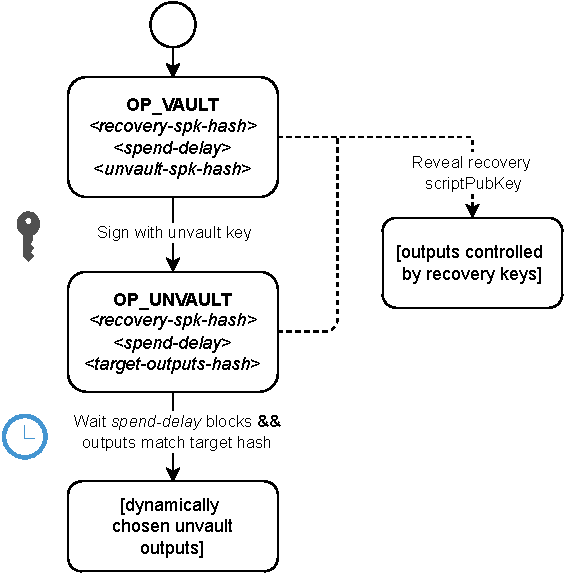
\includegraphics[width=0.5\linewidth]{op-vault.pdf}
  \centering
  \caption{A high-level description of the \opv{} state machine.}
\end{figure}

\subsection*{Components of the vault}

Each \opv{}-style vault makes use of a few pieces of essential data. These include

\begin{itemize}

  \begin{item}
    \textbf{a recovery path}: the destination that vault funds can be swept to
    at any point prior to the finalization of withdrawal to the \emph{unvault target}.

    This recovery address would usually correspond to a spending script that is
    inconvenient to exercise but is highly secure, e.g. a key generated offline or a
    geographically distributed multisig. It could be a P2TR address that incorporates a
    number of different spending conditions. 

    Vaults which share the same recovery path can be swept in batch operations, which
    is an important practical aspect of managing large numbers of vaults.

  \end{item}

  \begin{item} 
    \textbf{an unvault key}: used to authorize beginning an unvault process,
    i.e. the spending of an \opv{} into a suitable \opuv{}, which ``announces'' the
    intent to unvault and begins the withdrawal
    lock-in period. If an attacker obtains access to this key, the outcome is not
    catastrophic because any unvault can be interrupted and swept to the recovery
    address. 

    Vaults which have this in common can unvaulted in batch.
    
  \end{item}

  \item \textbf{an unvault target}: an arbitrary target or destination that is
    specified as a parameter to \opuv{}, and dictates where unvaulted funds go. This
    target consists of a list of destination outputs (including amounts) which the
    vault will be spent into after the delay period. These destinations can of course
    include recursive \opv{} outputs to facilitate partial-amount unvaults.

\end{itemize}

\subsection*{Initial vaulting}

To create a vault, a user would spend to an output with the following
\spk{} (or equivalent taproot structure):

\begin{minted}{sh}
  OP_VAULT <recovery-hash> <delay-period> <unvault-pk-hash> 
\end{minted}
\noindent where

\begin{itemize}
  \item \code{<recovery-hash>} is the SHA256 hash of the recovery \spk{}. This could
    e.g. correspond to a P2TR address with many spending conditions.

  \item \code{<delay-period>} is the number of blocks between when the \opuv{} confirms
    and when the funds can be spent to the unvault target outputs.

  \item \code{<unvault-pk-hash>} is the SHA256 hash of the public key whose signature is
    required to start the unvault process.

\end{itemize}

This output can only be spent one of two ways: 

\begin{enumerate}
  \item it can be swept to the recovery address at any point with no witness data, or
  \item it can be sent to an \opuv{} output matching the specification described
    below.
\end{enumerate}

\subsection*{Triggering an unvault}

To withdraw bitcoin from an \opv{}-encumbered output to some arbitrary destination, it
must first be spent into an \opuv{} output having a \code{scriptPubKey} of the form

\begin{minted}{sh}
  OP_UNVAULT <recovery-hash> <delay-period> <unvault-target-hash> 
\end{minted}

\noindent where the first two parameters are carried over from the input \opv{}
(described above), and
\emph{unvault-target-hash} is defined as

\begin{minted}{python}
  sha256d(sha256d(d.scriptPubKey) || sha256d(d.nValue) 
          for d in target_outputs)
\end{minted}

In other words, the target hash commits to the set of outputs that are proposing to be
withdrawn to. 

The unvaulting party must now wait a total of \emph{delay-period} blocks before being
able to broadcast a transaction spending the \opuv{} output into a set of outputs
satisfying \emph{unvault-target-hash}. No witness is needed for this finalizing
``withdrawal'' transaction.

If the owner of the vault does not recognize this proposed
withdrawal, he can sweep the vault into the recovery path before the delay period ends.


\subsection*{Sweeping to recovery}

In order to sweep an \opv{} or \opuv{} output to the recovery address, a transaction is
broadcast spending that output into a new output corresponding to the recovery address,
consuming the full amount of the output being swept. This can happen at any point
before withdrawal to the unvault target is finalized. 

The witness for the swept output is empty, since the only authorization necessary 
is simply that the \spk{} being spent to matches the \code{<recovery-hash>} committed
to in the parent \opv{} output.

\subsubsection*{Denial of service protection}

During the creation of \opv{} and \opuv{} outputs, the recovery address remains hidden
behind a hash. This avoids denial-of-service (DoS) attacks that involve a third party
attempting to blindly sweep vault transactions to their recovery path, which could
result in a temporary halt in liquidity while the vault owner goes through the
potentially lengthy process of activating the recovery keys for funds retrieval.

If it becomes necessary to make use of the recovery path, the recovery \spk{} will be
revealed, which means that any other vaults with that recovery path may be swept there
by an unauthenticated party. 

This seems like a reasonable trade-off, since presumably if the vault's owner
had to make use of the recovery path for one vault, any other vault sharing the
recovery path may be at risk due to a compromise in the owner's infrastructure.

\subsubsection*{Batching}

If multiple vaults share a common \emph{recovery-hash}, they can be swept in batch.
This is an especially important feature for users that maintain many vaults, since a key
compromise might necessitate the rapid sweeping of many vaults at once before a delay
period has elapsed. Batching the sweep reduces the chainspace required significantly,
because we're able to sweep to a total of two outputs instead of
creating \emph{2v} \footnote{An anchor output for fee control
is needed for each sweep transaction} 
outputs for \emph{v} vaults.

Note that this batching option is not possible in vault schemes that rely on limited,
i.e. precomputed, covenant techniques.

\begin{figure}[H]
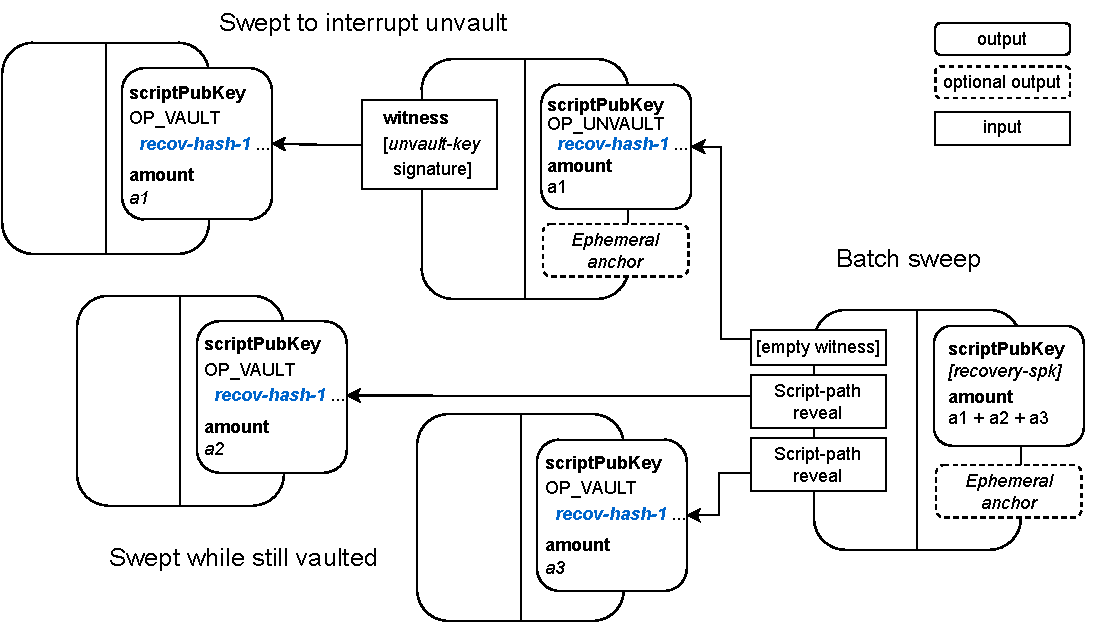
\includegraphics[width=0.9\textwidth]{batch-sweep.pdf}
\centering
\caption{Demonstration of multiple vaults being batch-swept simultaneously. Two of
  the vaults (bottom) are still vaulted while one (top) is interrupting an attempted unvault.}
\end{figure}

\subsection*{Managing fees safely}

One difficulty when designing this scheme was determining how to adjust the fee rate of
transactions that happen sometime after vault creation. The fee environment may be very
different during vault operations than when the vault was initially created; fees may
be much higher. 

The most common method of adjusting fee rate is to vary output
amounts, which leaves more bitcoin available to miners and thus adds to the
incentive to include a given transaction.
During an \opv{} lifecycle, allowing variable amounts would unfortunately
present some problems.

If an attacker discovers the recovery preimage, they may trigger undesired recovery
sweeps. If the \opv{} validation rules allowed output amounts to vary for the recovery
transaction, an attacker could simply set that value to 0 and burn the vaulted coins. 
A similar consideration must be applied to \opuv{} transactions.

In order to avoid such a failure, there are two options:

\begin{enumerate}
  \item script validation rules could require some allowable ``range'' of
    amount discounts during unvault/recovery to facilitate fee payment, or

  \item script vaildation rules could require that the unvault/recovery
    outputs preserve the full value of any vaults being acted on. 

\end{enumerate}
\emph{1.} seems like a bad design. \emph{2.} seems like the preferable approach, but it
introduces a complication: how are we to pay fees for sweep and
unvault transactions if the full value of the vaulted coins must be preserved?

\subsubsection*{Saved by package relay and ephemeral anchors}

Fee management is a thorny part of designing any contracting protocol built atop
Bitcoin script. Transactions which are presigned, or covenant structures that fix
amounts, cannot vary their amounts to adjust fees dynamically. A common workaround is
to attach an ``anchor output'' \cite{OptechAnchors}, which is an output that is
intended to be spent by some child transaction. Spending the child can raise the
effective feerate of its parent, the precommitted contract transaction. This is
referred to as child-pays-for-parent (CPFP).

This technique alone is insufficient for reliable fee control. If fees have risen
considerably since the initial contract negotiation and the feerate of a precommitted
transaction is beneath the minimum mempool feerate, it may be unable to broadcast in
the first place and CPFP cannot take place.

Luckily, it is looking increasingly likely that package relay policies
(\cite{OptechPkgRelay}) that remedy this will become part of bitcoin. The \opv{}
proposal detailed here not only assumes the presence of package relay, but also makes
use of \emph{ephemeral anchors} (\cite{Anchors}), zero-value outputs which must be 
spent within the package they're relayed with, in order to avoid unnecessarily wasting
vaulted value for fee control.

Our rationale for the permissibility of this hard dependency is that many -- perhaps
all -- contracting schemes built on Bitcoin become unworkable without a robust solution
for dynamic fee management, which itself appears to depend on package relay. We fully
expect that if \opv{} were found to be a desirable soft-fork, its deployment would
naturally come after the deployment of package relay and some kind of fee control
mechanism like ephemeral anchors.

Given the deploy of these modern facilities, the \opv{} strategy is able to both
provide efficient fee management and rule out coin-burning denial-of-service attacks.

\subsection*{Future-proofing fee control}

To avoid wasting value and to allow dynamic fee control, each \opuv{} transaction,
recovery sweep transaction, and unvault target transaction \emph{may} have an ephemeral
anchor output that facilitates robust fee management with CPFP and package relay.

But there are other possible designs for dynamic fee management. One is transaction
sponsors \cite{Sponsors}. Sponsors allow fee rate improvement of any unconfirmed
transaction by any party, and they do not require any structural ``awareness'' from the
transaction whose fee is being bumped. In the proposed design, sponsors would be
required by consensus to be mined alongside other transactions which they are
sponsoring. This allows CPFP-like adjustment of fee rate, but without a wasted output
or specific planning.

In order to allow for the possible adoption of such a proposal,
any ephemeral anchor outputs in the \opv{} scheme are strictly optional.

\section*{The importance of dynamic unvault targets}

In vault schemes which are usable today, the unvault target is always fixed at vault
creation time. Even in schemes that assume the use of a limited covenant mechanism like
CHECKTEMPLATEVERIFY or ANYPREVOUT, the set of withdrawal targets is similarly fixed.

The design presented here allows for the withdrawal target to be decided at unvault
time, before the delay period, rather than needing to be specified during the creation
of the vault. This presents a significant benefit, because if the withdrawal target is
fixed, an intermediary hot or warm wallet must be used to unvault and then send the
coins to their ultimate destination.

If a withdrawal target can be set at unvault time, no such intermediary wallet is
needed. This saves on operational complexity, avoids a potential avenue of compromise,
and also removes the need for an additional transaction -- which may be no small
consideration when considering possible future demand for chainspace.

\subsection*{Batching}

Dynamic unvault targets also allow for output amount adjustment that enables multiple
vaults to be unvaulted (or recovered) to a single set of output targets. This isn't
only important as blockspace becomes scarcer. After ruminating for some time on the
failure modes associated with vaults, the authors have become convinced that the
ability to recover or unvault as efficiently as possible is crucial
to thwarting an attacker.

\subsection*{Recursive deposits (revaults)}

Another benefit of supporting dynamic unvault targets is that an arbitrary number of
partial unvaults can happen by withdrawing to some output outside the vault, but then
redepositing some amount back into the same \code{OP\_VAULT ...} construction.

This could enable, for example, an exchange to offer a vault address to a customer,
allow them to make multiple deposits, and support partial withdrawals without having to
redo a vault initialization.

\section*{Downsides relative to other designs}

We have already written about the important benefits that this scheme provides relative
to alternatives. While we think the set of trade-offs for \opv{} are
appealing, it is important to acknowledge downsides.

A scheme that does not codify vault semantics at the script interpreter layer, e.g. one
that uses only a general covenant primitive like transaction introspection within
script, allows for more flexibility in the particular control flow of the vault, since
the rules of the vault are specified by the end-user instead of the consensus engine.
It more easily facilitates user experimentation.

For example, perhaps a user prefers to safeguard their recovery path with a
signature rather than revealing the preimage to a \spk{} hash, so that discovery of the
recovery path doesn't allow an unauthenticated user to sweep open vaults to recovery.

The downside, of course, is that this results in very large on-chain script sizes. In
order to make vault constructions concise, they ultimately must be codified in
validation rules, barring some breakthrough in a zero-knowledge proof system that could
be supported on-chain.

\section*{Conclusion}

We have presented a new set of opcodes, \opv{} and \opuv{}, which enable featureful
vaults in Bitcoin. These opcodes allow encumbering a set of coins in such a way that
their spending requires passing through a delay period, during which the coins can be
recovered to a set address. Enabling on-chain enforcement of such a control flow
presents significant benefits to custodians of bitcoin, whether large or small, because
in essence this scheme offers multisig-like security for an expected operational burden roughly
on par with single sig use.

The \opv{} proposal is unique in enabling robust dynamic fee management (thanks to
package relay and ephmeral anchors). It also enables batch management, a
critical feature when considering the need to respond to attackers efficiently and make
judicious use of chain space.


\section*{TODO}

- Mention operational considerations of running a watchtower

\printbibliography


\end{document}
